% !TEX TS-program = pdflatex
% !TEX encoding = UTF-8 Unicode
 
% This is a simple template for a LaTeX document using the "article" class.
% See "book", "report", "letter" for other types of document.
 
\documentclass[12pt]{report} % use larger type; default would be 10pt
 
\usepackage[utf8]{inputenc} % set input encoding (not needed with XeLaTeX)
 
%%% Examples of Article customizations
% These packages are optional, depending whether you want the features they provide.
% See the LaTeX Companion or other references for full information.
 
%%% PAGE DIMENSIONS
\usepackage{geometry} % to change the page dimensions
\geometry{a4paper} % or letterpaper (US) or a5paper or....
\geometry{margin=1in} % for example, change the margins to 2 inches all round
% \geometry{landscape} % set up the page for landscape
% read geometry.pdf for detailed page layout information
 
\usepackage{graphicx} % support the \includegraphics command and options
 
% \usepackage[parfill]{parskip} % Activate to begin paragraphs with an empty line rather than an indent
 
%%% PACKAGES
\usepackage{booktabs} % for much better looking tables
\usepackage{array} % for better arrays (eg matrices) in maths
\usepackage{paralist} % very flexible & customisable lists (eg. enumerate/itemize, etc.)
\usepackage{verbatim} % adds environment for commenting out blocks of text & for better verbatim
\usepackage{subfig} % make it possible to include more than one captioned figure/table in a single float
\usepackage{amsmath}
% These packages are all incorporated in the memoir class to one degree or another...
 \graphicspath{{Figures/}}
%%% HEADERS & FOOTERS
\usepackage{fancyhdr} % This should be set AFTER setting up the page geometry
\pagestyle{fancy} % options: empty , plain , fancy
\renewcommand{\headrulewidth}{0pt} % customise the layout...
\lfoot{}\cfoot{\thepage}
 
\rfoot{}
 
%%% SECTION TITLE APPEARANCE
\usepackage{sectsty}
\allsectionsfont{\sffamily\mdseries\upshape} % (See the fntguide.pdf for font help)
% (This matches ConTeXt defaults)
 
 
%%% END Article customizations
 
%%% The "real" document content comes below...
 
\title{\bf Example Project Document\\  }
\author{\bf Your Name
\\ Experimental Aerodynamics and Concepts Group
\\Daniel Guggenheim School of Aerospace Engineering
\\Georgia Institute of Technology
\\Atlanta GA 30332-0150
}
\date{\it Updated March 25, 2013} % Activate to display a given date or no date (if empty),
 
         % otherwise the current date is printed 

\usepackage{graphicx}
 
\begin{document}
\maketitle
 
\tableofcontents
 
\chapter{Abstract}

This document shell is assuming that the user has a basic understanding of using LaTeX including adding figures, equations , and citations and referencing them in the document to make a coherent document. 

\chapter{Introduction}
Add an introduction to the report here.

\chapter{Define Objectives}
 

{\bf Primary Objectives:} \\
\\ \\
{\bf Secondary Objectives:} \\
\\




\chapter{Prior Work}
Provide a literture survey of previous work done by you and others on this topic
\chapter{Project Schedule}
The project schedule should give dates of the projected time the task will be started and completed
\chapter{Experimental Setup}

\subsection{Model Details}
Give a full decription of your model, include all dimmentions in a computer animated drawing.



\subsection{Load Cell Details}

The wind tunnel has two options for the type of load cell you can choose. Please make a decision on the values given in the follwoing tables.
\\
\begin{table}[htbp]
  \centering
  \caption{Load Cell Selection: Sensing Ranges}
  \scalebox{1}{
    \begin{tabular}{llll}
    \hline
    \textbf{  } & \textbf{Calibration} & \textbf{Fx, Fy (lbf)} & \textbf{Fz (lbf)} \\
    \hline
    Delta &US-150-600&150&450 \\
     Gamma &US-30-100&30&100 \\
    \hline
    \end{tabular}
    }
  \label{tab:var}
\end{table}


\begin{table}[htbp]
  \centering
  \caption{Load Cell Selection: Sensing Ranges}
  \scalebox{1}{
    \begin{tabular}{llll}
    \hline
    \textbf{  } & \textbf{Calibration} & 
 \textbf{Tx, Ty (lbf-in)} & \textbf{Tz (lbf-in)}\\
    \hline
    Delta &US-150-600&600&600 \\
     Gamma &US-30-100&100&100 \\
    \hline
    \end{tabular}
    }
  \label{tab:var}
\end{table}

\begin{figure}[!ht]
\center

\begin{table}[htbp]
  \centering
  \caption{Load Cell Selection: Resolution}
  \scalebox{1}{
    \begin{tabular}{llll}
    \hline
    \textbf{  } & \textbf{Calibration} & \textbf{Fx, Fy (N)} & \textbf{Fz (N)} \\
    \hline
    Delta &US-150-600&1/16&1/8 \\
      Gamma &US-30-100&1/40&1/20 \\
    \hline
    \end{tabular}
    }
  \label{tab:va1r}
\end{table}


\begin{table}[htbp]
  \centering
  \caption{Load Cell Selection: Resolution}
  \scalebox{1}{
    \begin{tabular}{llll}
    \hline
    \textbf{  } & \textbf{Calibration} &  \textbf{Tx, Ty (Nm)} & \textbf{Tz (Nm)}\\
    \hline
    Delta &US-150-600&3/16&1/8 \\
      Gamma &US-30-100&1/800&1/800 \\
    \hline
    \end{tabular}
    }
  \label{tab:va1r}
\end{table}


\begin{figure}[!ht]
\center
\includegraphics[width =14cm,height = 16cm natwidth = 640, natheight = 480]{comp_len.png}
     \caption{Delta load cel specs}
     \label{fig:Delta load cel specs}
\end{figure}

\begin{figure}[!ht]
\center
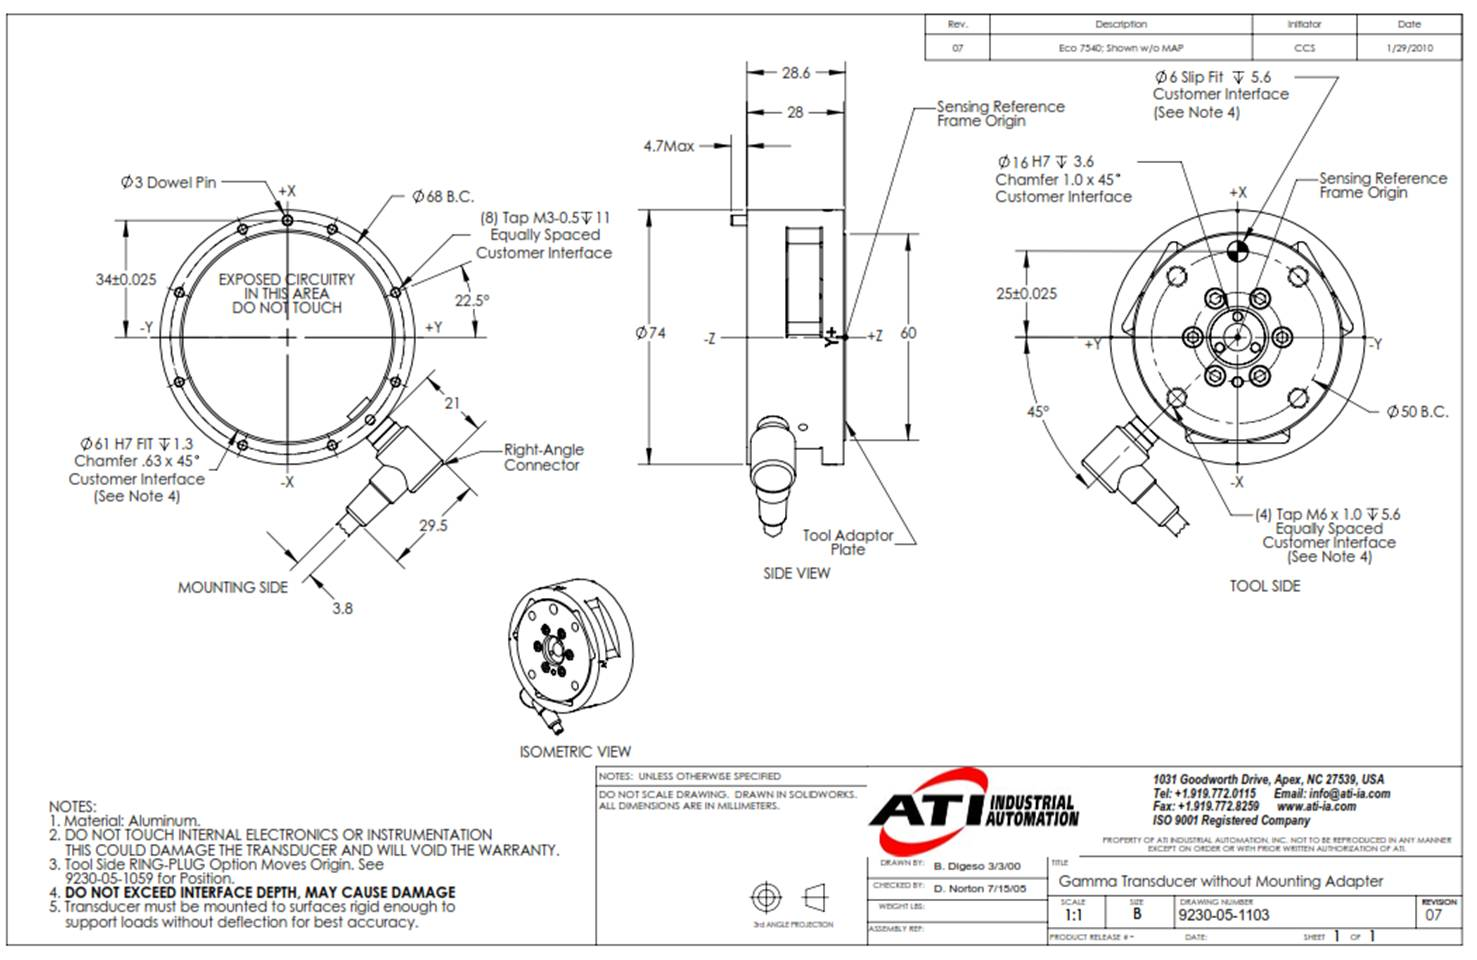
\includegraphics[width = 140mm]{Gamma.jpg}
     \caption{Gamma load cell specs}
     \label{fig:Gamma load cel specs}
\end{figure}





\subsection{Calculations of expected forces and moments}

\subsection{Static testing of the model}


\chapter{Flow and Test Conditions}

Add here what are the flow conditions and test conditions you want to run the experiments at. 
\\\\\
For example - Reynolds number sweep, or angle of attack sweep etc. The best would be to use a matrix of test runs so that it can be optimized to reduce the number of runs.

\begin{table}[htbp]
  \centering
  \caption{Test Matrix}
  \scalebox{1}{
    \begin{tabular}{llll}
    \hline
    \textbf{Run} & \textbf{Reynolds Number} & \textbf{Wind Tunnel Fan RPM}&\textbf{Angle of Attack (deg)} \\
    \hline
&&& \\
    
    \hline
    \end{tabular}
    }
  \label{tab:var}
\end{table}


\chapter{Expected results and plots}


\chapter{Conclusions}


\begin{thebibliography}{9}
\bibitem[Doe]{doe} \emph{First and last \LaTeX{} example.},
John Doe 50 B.C. 
\end{thebibliography}


\end{document}
